\documentclass[conference]{IEEEtran}
\IEEEoverridecommandlockouts
% The preceding line is only needed to identify funding in the first footnote. If that is unneeded, please comment it out.
\usepackage{cite}
\usepackage{amsmath, amssymb, amsfonts}
\usepackage{algorithmic}
\usepackage{graphicx}
\usepackage{textcomp}
%\usepackage{fourier} % fuck, but I like that font :(
\usepackage{libertinust1math} % - cool one
%\usepackage{MnSymbol}
\usepackage[english]{babel}
\usepackage[fixlanguage]{babelbib}
\usepackage[unicode=true,hidelinks]{hyperref}

\begin{document}

\renewcommand*{\figureautorefname}{Fig.}
\renewcommand*{\equationautorefname}{Eq.}

\def \w{\omega}

% ------------------------- %

\def \eq{\begin{equation}}
\def \qe{\end{equation}}
\def \eqc{\begin{equation*}}
\def \cqe{\end{equation*}}

% ------------------------- %
% ------------------------- %

\newcommand{\shifthat}[2]{%
    \stackengine{\Sstackgap}{$#2$}{\(\hspace{#1}\hat{}\)}{O}{l}{F}{T}{S}
}

% ------------------------- %

\newcommand{\operator}[2][operator]{
    \if H#2\shifthat{0.5em}{#2}\else
    \if d#2\shifthat{0.49em}{#2}\else
    \if q#2\shifthat{0.35em}{#2}\else
    \if \mu#2\shifthat{0.35em}{#2}\else
    \shifthat{0.45em}{#2}
    \fi
    \fi
    \fi
    \fi
}

% ------------------------- %

\newcommand{\vectoperator}[2][operator]{
    \if d#2\shifthat{0.367em}{\textbf{#2}}\else
    \if m#2\shifthat{0.4em}{\textbf{#2}}\else
    \shifthat{0.275em}{\textbf{#2}}
    \fi
    \fi
}

% ------------------------- %

\newcommand{\vect}[3][vector]{
    \overrightarrow{#2_{#3}}
}

% ------------------------- %

\newcommand{\vectbf}[2][bold vector]{
    \vect{\textbf{#2}}
}

% ------------------------- %

\newcommand{\pd}[3][empty]{
    \frac{\partial {#2}}{\partial {#3}}
}

% ------------------------- %

\newcommand{\func}[5][empty]{
    {#2}_{#3}^{#4} \left({#5} \right)
}

% ------------------------- %

\newcommand{\underrel}[3][]{
    \mathrel{\mathop{#3}\limits_{
        \ifx c#1\relax\mathclap{#2}\else#2\fi
    }}
}
% ------------------------- %

\makeatletter

\newcommand{\Autoref}[1]{\@first@ref#1,@}
\def\@throw@dot#1.#2@{#1}% discard everything after the dot
\def\@set@refname#1{%    % set \@refname to autoefname+s using \getrefbykeydefault
    \edef\@tmp{\getrefbykeydefault{#1}{anchor}{}}%
    \xdef\@tmp{\expandafter\@throw@dot\@tmp.@}%
    \ltx@IfUndefined{\@tmp autorefnameplural}%
        {\def\@refname{\@nameuse{\@tmp autorefname}}}%
        {\def\@refname{\@nameuse{\@tmp autorefnameplural}}}%
}
\def\@first@ref#1,#2{%
\ifx#2@\autoref{#1}\let\@nextref\@gobble% only one ref, revert to normal \autoref
\else%
    \@set@refname{#1}%  set \@refname to autoref name
    \@refname\ref{#1}% add autoefname and first reference
    \let\@nextref\@next@ref% push processing to \@next@ref
\fi%
\@nextref#2%
}
\def\@next@ref#1,#2{%
\ifx#2@,~\ref{#1}\let\@nextref\@gobble% at end: print and+\ref and stop
\else, \ref{#1}% print  ,+\ref and continue
\fi%
\@nextref#2%
}

\makeatother

% ------------------------- %
% ------------------------- %

\newcommand{\img}[4][anything]{
    \begin{figure}[H]{
        \center{\includegraphics[width={#4}]{{#1}}}
        \caption{#2}\label{#3}}
    \end{figure}
}

% ------------------------- %

\newcommand{\floatimg}[4][anything]{
    \begin{figure}[ht]{
        \center{\includegraphics[width={#4}]{{#1}}}
        \caption{#2}\label{#3}}
    \end{figure}
}

% ------------------------- %

\newcommand{\subimg}[2][anything]{
    \begin{minipage}[h]{{#2}} % 0.4\textwidth
        \center{\includegraphics[width=1\linewidth]{{#1}}}
    \end{minipage}
}

% ------------------------- %

\newcommand{\subimgtwo}[4][anything]{
    \subfloat[{#2}]{\includegraphics[width={#4}]{{#1}}\label{#3}}
}

% ------------------------- %

\title{Angular dispersion boost of high order laser harmonics interacting with dense plasma clusters}
% {\footnotesize \textsuperscript{*}\textit{Note: Sub-titles are not captured in Xplore and
% should not be used (this footnote should be deleted)}}
% \thanks{Identify applicable funding agency here. If none, delete this.}
% }

\author{
	\IEEEauthorblockN{L.\,A. Litvinov\textsuperscript{1}, A.\,A. Andreev\textsuperscript{1, 2}}
	\IEEEauthorblockA{\textsuperscript{1}Saint Petersburg State University, Saint Petersburg, Russia}
	\IEEEauthorblockA{\textsuperscript{2}Ioffe Physico-Technical Institute, Saint Petersburg, Russia}
}


\maketitle

\begin{abstract}% which is 
	 We propose a nanosphere array target in the plasma phase as an efficient dispersive medium for the intense XUV light originated from laser-plasma interactions where various high harmonic generation processes take place. The scattering process is studied with the help of numerical simulations using resonance conditions obtained from the analytical model. We show that the angular distribution of different harmonics after scattering can be good described by a simple interference, in particular for the rectangle symmetry the angular distribution corresponds to the Bragg-Wolfe diffraction theory.
\end{abstract}

\begin{IEEEkeywords}
	XUV light diffraction, ionized cluster gas, femtosecond laser plasma
\end{IEEEkeywords}

%\section{Introduction}

Limited size targets interacting with intense coherent light is well-studied phenomenon of linear excited surface plasmonic oscillations. Exciting of surface plasmons can lead to significant boost internal and external field on cluster eigenfrequency, that can cause enhancement of scattered field at large angles relative to the direction of incident wave.

Periodic surface gratings or photonic crystals are excellent tools for light diffraction and direction. However, this method is less effective in the case of extreme ultraviolet (XUV) light due to the high absorption of any material in this frequency range. Within the present work we research the possibility of angluar boost of a radiation in the XUV range by scattering on suitable spherical clusters.

%\section{Base model}

Similar to the work~\cite{andreev_lecz} we develop analytical model for a single cluster based on the Drude dielectric function of the plasma and the Mie scattering theory. The model was constructed in the quasi-static approximation since the ionization time is shorter than the pulse duration, which is much shorter than the plasma expansion time: femtosecond pulse of Ti:Sa laser with wavelength $\lambda_{L} = 830$ nm is in considering, the high harmonics beam generated by a nonlinear medium and the 10th harmonic filtered.

To investigate the resonance conditions the determination of the scattering coefficients is necessary in general. Since we are only interested in particle sizes smaller than the incident wavelength we use the limiting forms of the Bessel functions~\cite{boren_huffman}. Such approximations allow us to estimate the resonance parameters for a target with pre-defined wavelength, in particular the resonance electron density and the radius. In first-order approximation with wavelength $\lambda_{10} = \lambda_{L} / 10 = 83$ nm we need $n_e \approx 5.7 \cdot 10^{23}$ $\textrm{cm}^{-3}$ for $ka = 0.7$ ($a \approx 8.91$ nm) to reach efficient scattering.

With these parameters of single cluster target we consider the resonance and non-resonance case, corresponding to the 1st and 10th harmonic. We found a good scattered field enhancement (about 5 times) in the resonance case in comparison with the non-resonance case.

%\section{Simulations}

%\subsection{Scattering by an array}

Using the same resonance conditions for a single cluster, we simulate diffraction by an array of such clusters using code CELES~\cite{celes}.


% ------------------------

% Diffraction orders can be obtained with Bragg's law \cite{kress_bernard}.

% According to Bragg's law we obtain $\theta = \arcsin\frac{1}{4}$ for grating with $d = 2\lambda$ and $\theta = \arcsin\frac{1}{6}$ for grating with $d = 3\lambda$ in $1$-st diffraction order. Using these values we numerically compute the scattered field of 10-th laser harmonic with wavelength $\lambda_{10} = 83$ nm.

% We can see directions corresponding to the angular boost of the incident beam, in particular, for $d = 2\lambda_{10}$ there are two fairly clear directions.

\begin{figure}[htbp]
	\centerline{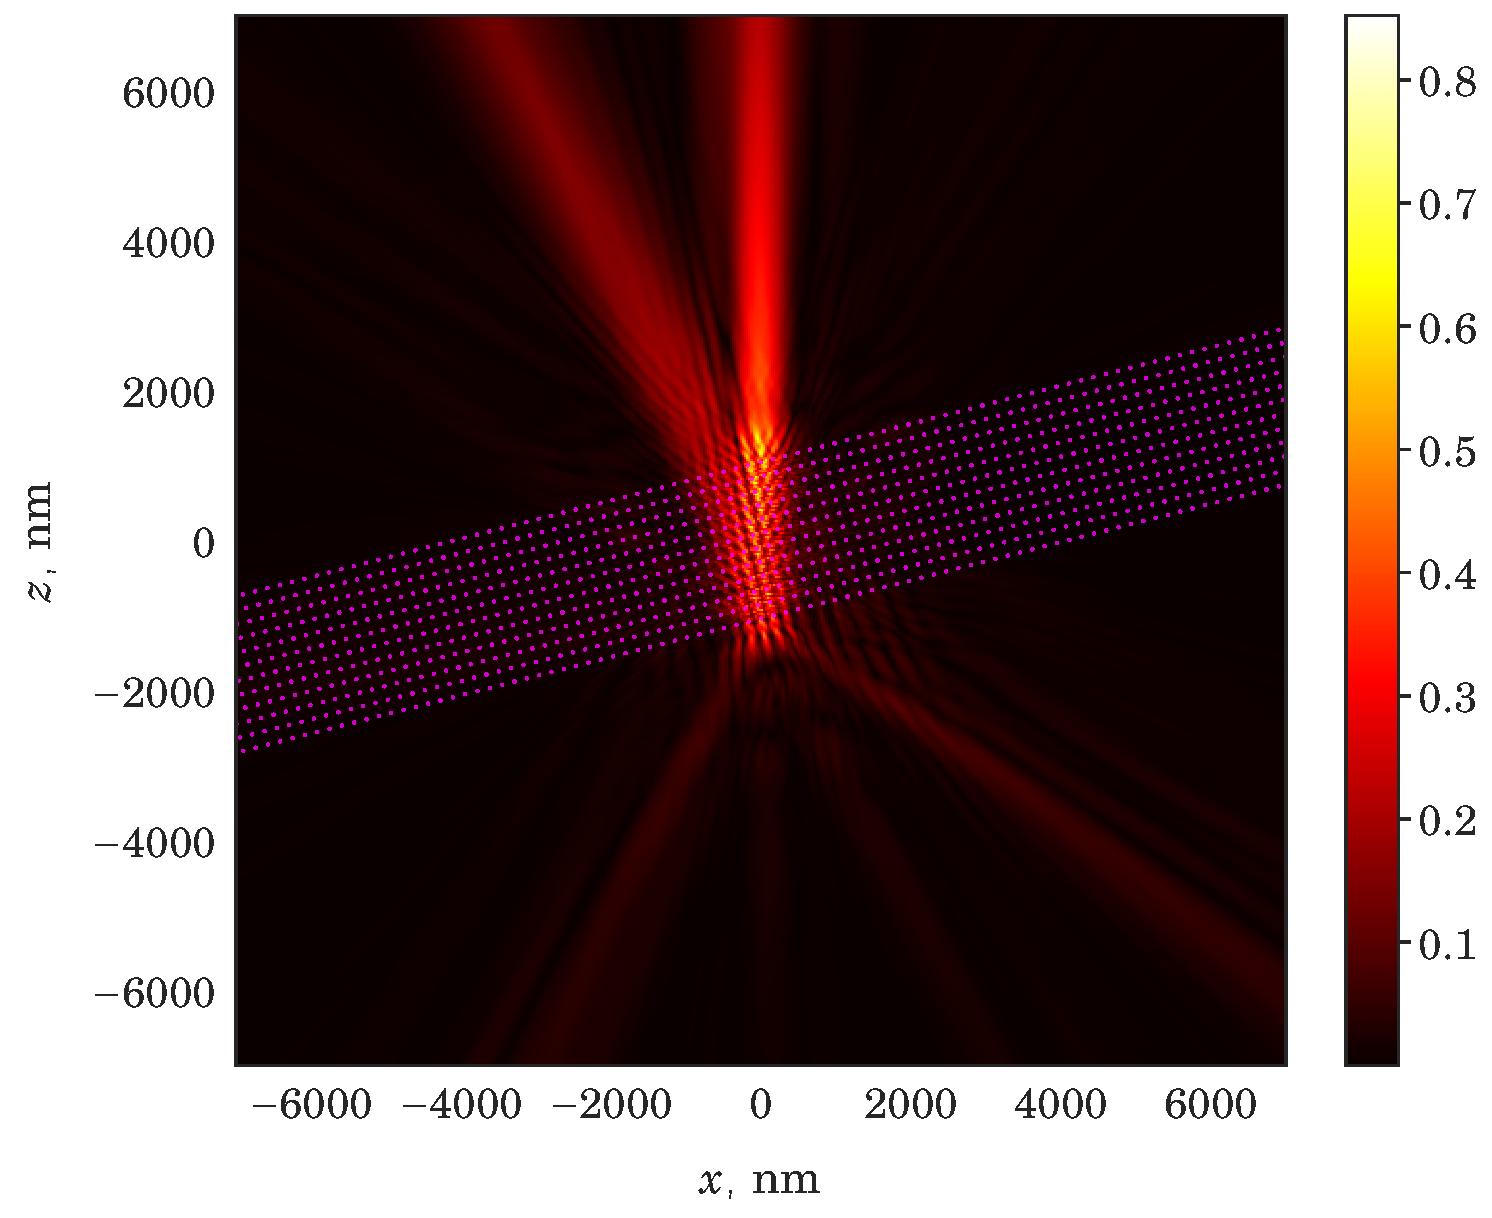
\includegraphics[width=0.71\columnwidth, trim={0 0.15cm 0 0.2cm},clip]{../components/img/celes/TE_14.324deg_check.pdf}}
	\caption{Scattered electric field normalized by the incident beam amplitude. The incident field represented by the gaussian beam with width $w = 850$ nm, $x$-polarized, propagating along positive direction of $z$ axis; the incident angle $\theta = 14.324^{\circ}$, the distance between clusters $d = 2\lambda_{10}$.}
	\label{14.324deg:image}
\end{figure}

At \autoref{14.324deg:image} zero and first diffraction order can be
observed, also there is weak second and minus first order of the reflected light. From the amplitude of the electric field in the first-order diffraction it can be assumed about 30\% of the radiation volume is directed. A configuration with a random deviation of the cluster positions within 20\% of the radius $a$ was also calculated. The direction of the first diffraction maximum changed slightly.

Obtained results show a significant boost of the scattered field in the resonance case for large angles, which corresponds to the Bragg-Wolfe diffraction theory~\cite{boren_huffman}, --- the ability to control high harmonics of laser radiation in XUV range using an ionized cluster gas.

\selectbiblanguage{english}
\bibliographystyle{ieeetr}
\bibliography{../components/bibliography.bib}

\end{document}
